\section{Детали реализации компонент платформы}
\label{sec:dev-details}

\subsection{Кастомизация SharpDevelop}
\label{sec:sd_custom}

Среда разработки SharpDevelop имеет встроенный механизм поддержки плагинов~\cite{sharpdevelop}. Более того, ядро IDE представляет из себя всего лишь платформу для поддержки плагинов~\cite{use-sd-core}, частью которой и является SDA, рассмотренная ранее. Функционал SharpDevelop реализуется при помощи целой иерархии взаимосвязанных плагинов, хранящихся в папке {\it \\AddIns}. Каждый плагин имеет свой собственный xml-файл конфигурации {\it *.addin}, в котором размещается информация, необходимая ядру для интеграции плагина~\cite{writing-sd-addin}. 

Помимо отдельных конфигурационных файлов для каждого плагина, существует отдельно лежащий конфигурационный файл {\it ICSharpCode.SharpDevelop.addin}. Этот файл определяет поведение сборки {\it ICSharpCode.SharpDevelop.dll}, которая сама по себе так же является плагином, но очень крупным. Можно сказать, что эта сборка и реализует базовый функционал IDE.

В файле содержится несколько секций, рассмотрим подробно те, которые будут использоваться для кастомизации: 

\begin{itemize}
 \item <AddIn> Заголовочная секция, содержит имя сборки, описание, автора, а так же определяет видимость в менеджере плагинов(видимый через менеджер плагин можно отключить)
 \item <Manifest> Хранит имя и версию сборки
 \item <Runtime> <Import> Определяет сборки, загружаемые ядром.
 \item <Path> Содержит путь к визуальному элементу управления типа <<контейнер>>. Внутри этой секции располагается описание различных элементов, которые находятся в контейнере, а так же их поведение.
   \subitem <MenuItem>, <ToolbarItem> Элементы управления. Могут содержать информацию о связаных ресурсах (иконка, текст, всплывающая подсказка), а так же имя класса-обработчика.
   \subitem <Condition>, <ComplexCondition> Условие, либо составное условие, описывающее будет ли отображаться тот или иной элемент управления в определенных ситуациях.
\end{itemize}

Таким образом при помощи конфигурационных файлов можно реализовать несколько сценариев кастомизации:

\begin{itemize}
 \item Загрузка дополнительных сборок в адресное пространство SharpDevelop
  \subitem с целью подменять обработчики событий существующих элементов управления на свои собственные;
  \subitem с целью создания своих собственных элементов управления различного типа (кнопки, панели инструментов, пункты меню, и т. д.)
 \item Комментирование кода в конфигурационном файле для удаления ненужных элементов управления или выключения загрузки сборок.
 \item Добавление или изменение условий.
\end{itemize}
 
Помимо перечисленных сценариев кастомизации SharpDevelop и его компонент с использованием конфигурационных файлов, есть возможность реализации плагинов для этой среды разработки. В рамках этой работы создание плагинов рассматриваться не будет, так как все необходимые действия удалось совершить при помощи конфигурационного файла.
 
Для решения задачи кастомизации была создана библиотека, содержащая обработчики следующих событий SharpDevelop (в скобках указано новое действие):

\begin{itemize}
 \item Создание нового проекта (вызывает соответствующий диалог создания расширения);
 \item Открытие существующего проекта (диалог открытия проекта расширения из файла/базы данных/архива);
 \item Сохранение проекта/файла (диалог сохранения проекта в файл/базу данных/архив);
 \item Сборка проекта (в случае успешной сборки, обработчик готовит исполняемый файл расширения к загрузке в адресное пространство приложения);
 \item Старт отладки (загружает файл расширения в адресное пространство приложения и присоединяет к его процессу встроенный в SharpDevelop отладчик);
\end{itemize}

Эти события требуют интеграции в хост-процесс IDE для обеспечения взаимодействия с расширяемым приложением. Реализация своих собственных обработчиков требовала детального изучения исходного кода и архитектуры SharpDevelop, для обеспечения стабильности такого решения. Пример исходного кода обработчика с комментариями можно найти в приложении ?; фрагменты измененного файла конфигурации {\it ICSharpCode.SharpDevelop.addin} см. приложение ?.
 
 %-----------------------------------------------------------------
 
\subsection{Управление сборками расширений}
\label{sec:dll_manip}

Один из сценариев использования платформы --- редактирование кода расширения. При этом подразумевается, что отредактированный проект расширения будет перекомпилирован и обновленный бинарный файл будет загружен в адресное пространство расширяемого приложения. При этом возникает несколько проблем:

\begin{itemize}
  \item Необходимо так же загружать {\it .pdb} файлы, содержащие информацию для отладчика.
  \item После загрузки библиотеки приложением, она более не может быть выгружена из домена приложения, соответственно файл библиотеки блокируется.
  \item Необходимо, чтобы компилятор среды SharpDevelop всегда мог перезаписать библиотеку расширения после ее компиляции.
\end{itemize}

Теоретически, для организации работы с файлами библиотек может быть использовано несколько подходов:

\begin{itemize}
  \item Загрузка бинарного файла и отладочной информации в домен приложения в виде потока байт {\it MemoryStream}.
  При этом подходе файл библиотеки не блокируется приложением и может быть повторно перезаписан при последующих сборках расширения. Однако при попытке использования такого подхода оказалось, что отладчик SharpDevelop не умеет подгружать отладочную информацию из потока байт. От этого способа пришлось отказаться.
  \item Копирование бинарного файла и отладочной информации в специально отведенное для этого хранилище, из которого они, в свою очередь, будут загружены в приложение.
  Существует как минимум два варианта реализации этого подхода.
    \subitem Хранение всех версий сборок в одной папке в виде файлов с уникальным случайным именем. Такой способ так же не принес результатов, так как и в этом случае отладчик SharpDevelop отказался находить отладочную информацию.
	\subitem Создание для каждой версии сборки своей временной папки. Наконец, в этом случае с отладчиком не возникло проблем, и было решено использовать именно такой сценарий хранения файлов расширений.
\end{itemize}

Для реализации задачи хранения сборок было решено использовать изолированное хранилище. Оно имеет определенные преимущества по сравнению с другими возможными способами организации хранения. Во-первых, изолированное хранилище доступно даже, если у пользователя нету привилегий в файловой системе. Во-вторых, оно достаточно хорошо скрыто от посторонних глаз в профиле пользователя. Наконец, для реализации работы с изолированным хранилищем в .NET существует объект {\it IsolatedStorageFile}. Он служит для создания различных файлов и папок в изолированном хранилище и проведения манипуляций с ними. После окончания работы с программой, изолированное файлы в хранилище могут быть удалены, или же оставлены. При этом гарантирована их доступность при повторном запуске приложения. В данном случае, временные сборки не представляют интерес, и будут удаляться по завершению работы с приложением.

 %-----------------------------------------------------------------
 
\subsection{Интеграция с отладчиком}
\label{sec:sd_debug}

В процессе тестирования отладчика скриптов, стало понятно, что работать с ним не очень удобно. Основная причина этого заключалась в том, что при остановке выполнения скрипта на точке останова поток приложения, в котором выполняется этот скрипт блокируется, но при этом больше никаких действий не происходит, в худшем случае пользователь видит <<зависшее>> приложение. То есть пользователю каждый раз, когда приложение <<зависает>>, приходится переключаться на окно IDE и проверять, не остановилось ли выполнение скрипта отладчиком. Такое поведение недопустимо. Необходимо, чтобы при остановке на брейкпоинте окно SharpDevelop сообщало об этом, например, его статус бы менялся на <<Поверх всех окон>>.

Казалось бы, для реализации подобного поведения необходимо изменить код SharpDevelop, добавив в событие точки останова <<BreakpointHit>> код для изменения статуса главного окна. Однако, изменение исходного кода повлекло бы за собой проблемы при распространении платформы, которая не могла бы использовать существующий инсталляционный пакет SharpDevelop, а требовала установки модифицированной его версии. Это так же неудобно, если пользователь собирается использовать SharpDevelop для других целей. Такое изменения поведения в этом случае нежелательно.

Задача изменения реакции на внутреннее событие была решена при помощи рассмотренного ранее механизма {\it .NET Reflection}~\cite{CLR-via-CS}. Ниже приведены фрагменты кода класса {\it SDBreakpointService} с комментариями.

Объявление дополнительного обработчика события достижения точки останова:

\begin{lstlisting}
var bpDebuggerBreakpointHit 
     = new EventHandler<Debugger.BreakpointEventArgs>(
        delegate
        {
              SDIntegration.Instance.BringToFrontIDE();
        }
);
\end{lstlisting}


Получение коллекции точек останова, установленных в открытом проекте:	

\begin{lstlisting}
var fieldInfo = DebuggerService.CurrentDebugger.GetType().GetField(
      "debugger", BindingFlags.Instance | BindingFlags.NonPublic);
var debugger = fieldInfo.GetValue(DebuggerService.CurrentDebugger);
var field = debugger.GetType().GetField("breakpointCollection", 
     BindingFlags.Instance | BindingFlags.NonPublic);
var breakPointColl = (IEnumerable)field.GetValue(debugger);
\end{lstlisting}

Как видно, здесь происходит обращение к закрытым членам класса {\it Debugger} из плагина {\it Debugger.Core.dll}. Это нужно учитывать при миграции платформы на следующие версии SharpDevelop, так как логика работы этого класса может измениться.

Далее, всем точкам останова присваивается дополнительный обработчик события:

foreach (var bp in breakPointColl)
{
	bp.GetType().GetEvent("Hit").AddEventHandler(bp, bpDebuggerBreakpointHit);
}

Стоит отметить, что эти действия необходимо повторять для каждого нового брейкпоинта, установленного в IDE. К счастью, событие установки брейкпоинта существует, и доступно <<из коробки>>, поэтому дополнительных проблем с этим не возникло.

Так же стоит отметить, что в SharpDevelop начиная с версии 4.1 наконец-то появилась опция автоматической остановки выполнения приложения с подключенным отладчиком в случае возникновения исключительной ситуации. Благодаря этой функции разработчику расширения будет понятно, в каком месте кода произожло исключение. Напомню, в ранних версиях SharpDevelop (4.0 и ниже) такой возможности не было, и в случае необработанного исключения приложение просто завершилось бы с ошибкой. В такой ситуации исправлять ошибки в коде расширения довольно затруднительно. 

 %-----------------------------------------------------------------

\subsection{Реализация генератора сигнатур обработчиков событий}
\label{sec:ehsg}

\begin{figure}[!h]
    \centering
    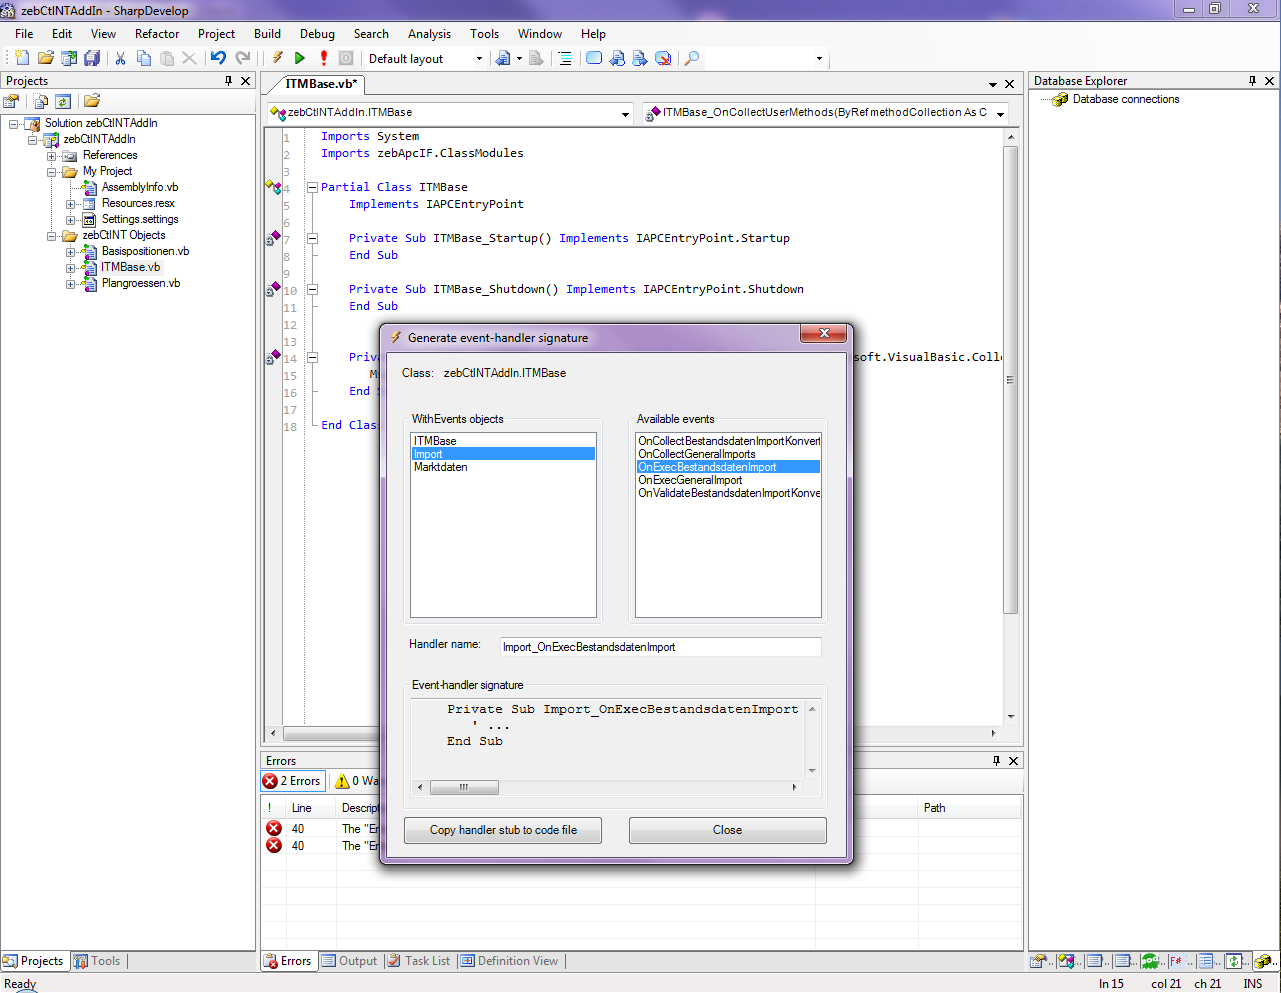
\includegraphics[width=16cm]{sdesg.png}
    \caption{Пример работы с генератором обработчиков сигнатур}
    \label{pic:sdesg}
\end{figure}

 %-----------------------------------------------------------------

\subsection{Реализация пользовательского интерфейса управления расширениями}
\label{sec:macro-gui}



\begin{figure}[!h]
    \centering
    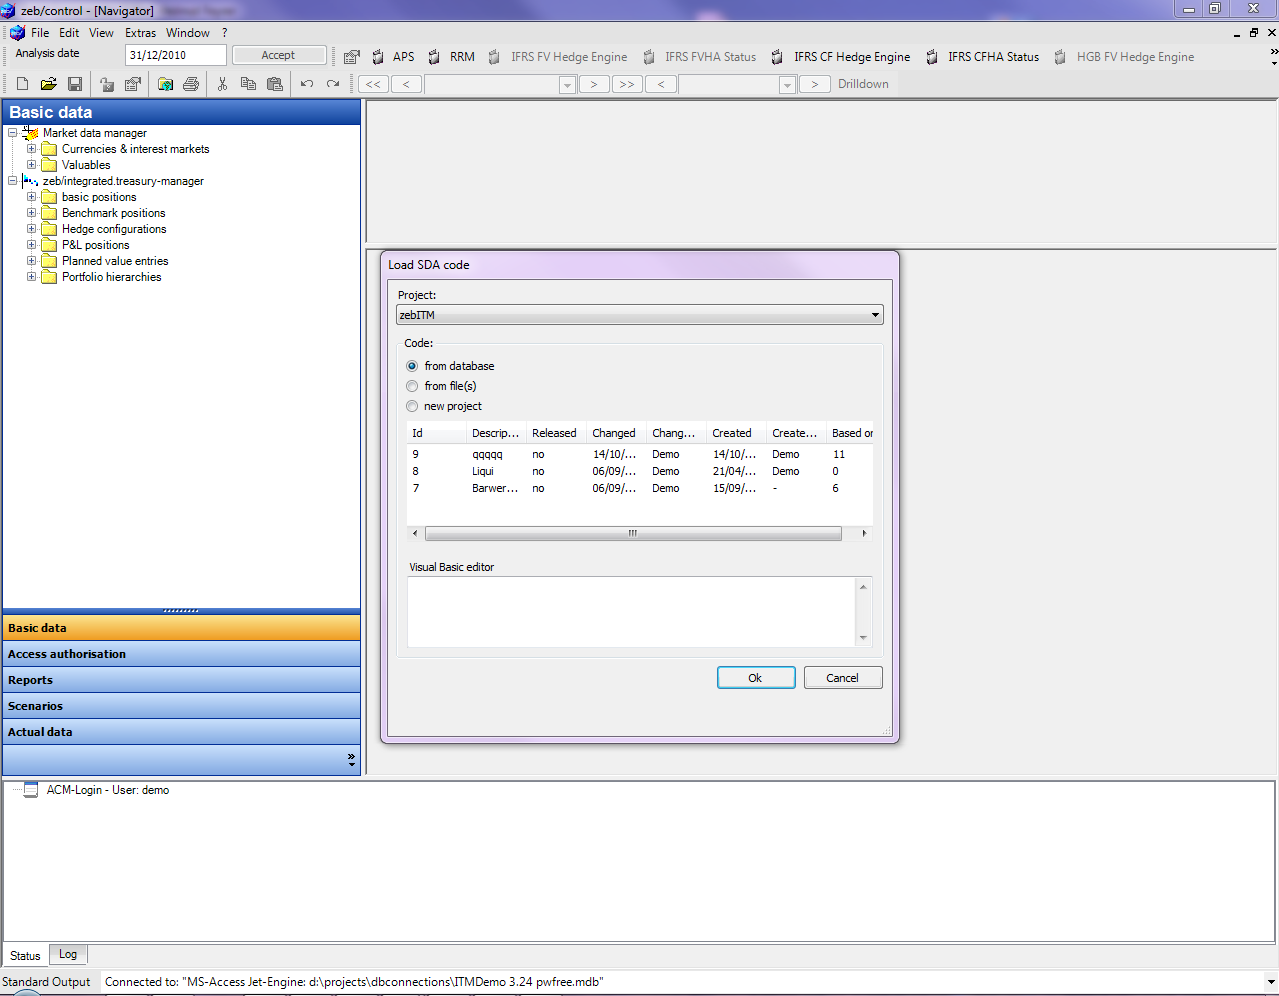
\includegraphics[width=16cm]{mmui.png}
    \caption{Главное окно приложения, в которое интегрирована разработанная платформа. Открыто окно загрузки расширения}
    \label{pic:mmui}
\end{figure}

 %-----------------------------------------------------------------

\subsubsection{Организация доступа к объектам приложения}
\label{sec:ext_entry_point}

\ref{pic:ext_design}

\begin{figure}[!h]
    \centering
    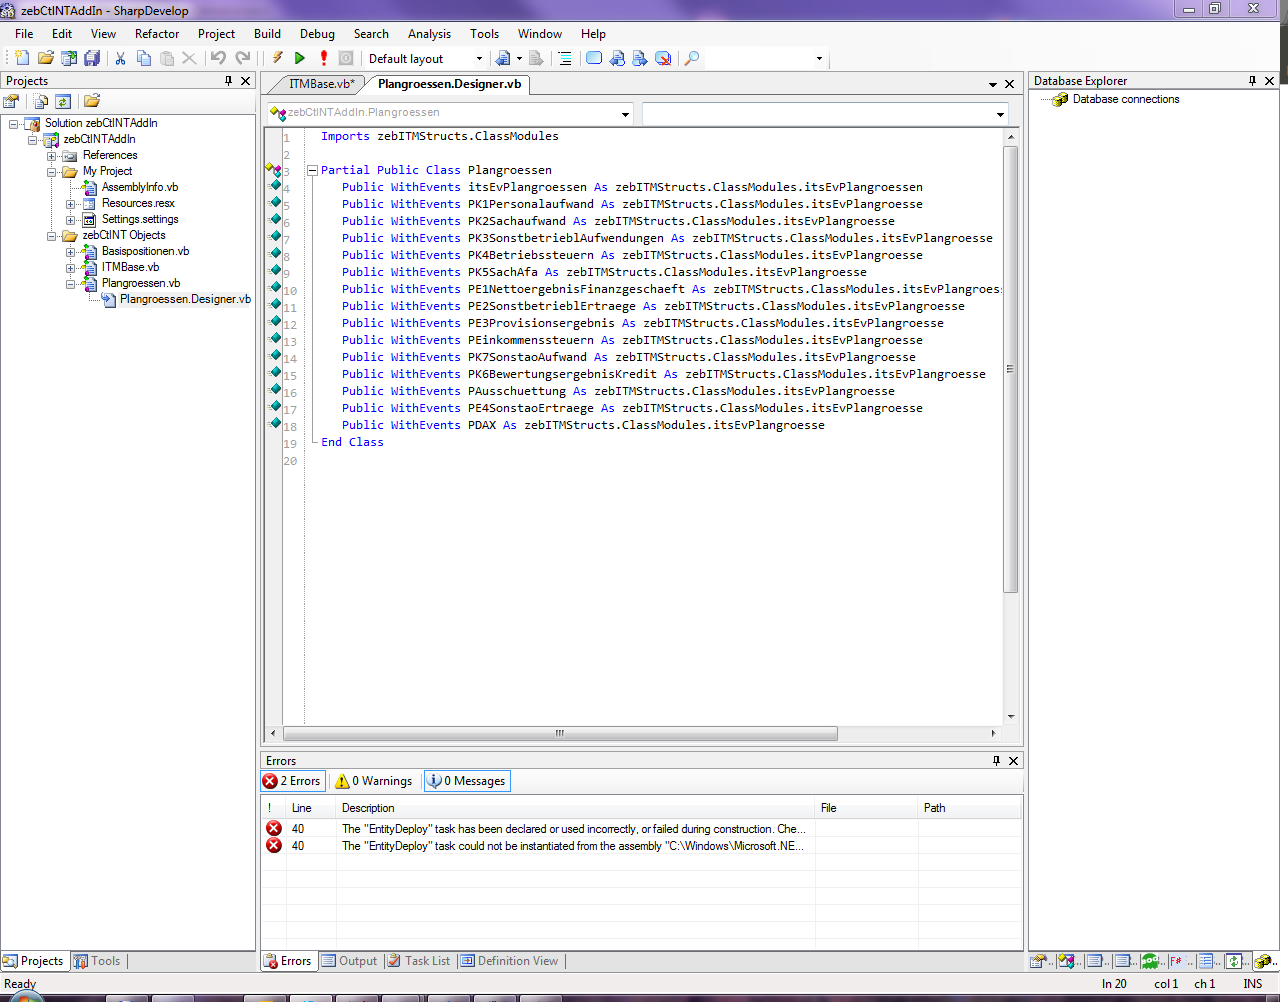
\includegraphics[width=16cm]{ext-design.png}
    \caption{Один из дизайн-файлов макропроекта, открытого в SharpDevelop}
    \label{pic:ext_design}
\end{figure}
 
\subsection{Улучшение общей отказоустойчивости системы}
\label{sec:stability}

В процессе тестирования платформы на реальном проекте была отмечена довольно низкая общая надежность связки <<Приложение --- хост-процесс IDE --- SharpDevelop>>. Так как бесперебойная работа системы зависит от корректного выполнения сразу двух процессов, а так же безошибочного обмена данными между ними, общая отказоустойчивость понижается, так как отказ в любом месте системы приводит к ее полному краху. Логично, что чем больше зависимых компонент в системе, тем менее стабильно она работает. Решить проблему можно либо повышая стабильность каждого из узлов системы, для снижения вероятности отказа, либо реализации возможности корректного восстановления работы компонента в случае его отказа. Хорошим решением является применение обоих вариантов одновременно.

Чтобы повысить общую отказоустойчивость было решено внедрить механизм автоматического восстановления корректной работы хост-процесса IDE и канала связи между процессами в нештатных ситуациях.

В случае ошибки в хост-процессе, он <<сообщает>> об этом приложению и перезапускается. При этом обмен данными приостанавливается до полного восстановления работоспособности каналов обмена. При обрыве канала так же происходит его переинициализация.

\pagebreak